% Options for packages loaded elsewhere
\PassOptionsToPackage{unicode}{hyperref}
\PassOptionsToPackage{hyphens}{url}
\PassOptionsToPackage{dvipsnames,svgnames,x11names}{xcolor}
%
\documentclass[
  10pt,
  a4paper,
  DIV=11,
  numbers=noendperiod]{scrreprt}

\usepackage{amsmath,amssymb}
\usepackage{iftex}
\ifPDFTeX
  \usepackage[T1]{fontenc}
  \usepackage[utf8]{inputenc}
  \usepackage{textcomp} % provide euro and other symbols
\else % if luatex or xetex
  \usepackage{unicode-math}
  \defaultfontfeatures{Scale=MatchLowercase}
  \defaultfontfeatures[\rmfamily]{Ligatures=TeX,Scale=1}
\fi
\usepackage{lmodern}
\ifPDFTeX\else  
    % xetex/luatex font selection
\fi
% Use upquote if available, for straight quotes in verbatim environments
\IfFileExists{upquote.sty}{\usepackage{upquote}}{}
\IfFileExists{microtype.sty}{% use microtype if available
  \usepackage[]{microtype}
  \UseMicrotypeSet[protrusion]{basicmath} % disable protrusion for tt fonts
}{}
\makeatletter
\@ifundefined{KOMAClassName}{% if non-KOMA class
  \IfFileExists{parskip.sty}{%
    \usepackage{parskip}
  }{% else
    \setlength{\parindent}{0pt}
    \setlength{\parskip}{6pt plus 2pt minus 1pt}}
}{% if KOMA class
  \KOMAoptions{parskip=half}}
\makeatother
\usepackage{xcolor}
\setlength{\emergencystretch}{3em} % prevent overfull lines
\setcounter{secnumdepth}{5}
% Make \paragraph and \subparagraph free-standing
\ifx\paragraph\undefined\else
  \let\oldparagraph\paragraph
  \renewcommand{\paragraph}[1]{\oldparagraph{#1}\mbox{}}
\fi
\ifx\subparagraph\undefined\else
  \let\oldsubparagraph\subparagraph
  \renewcommand{\subparagraph}[1]{\oldsubparagraph{#1}\mbox{}}
\fi


\providecommand{\tightlist}{%
  \setlength{\itemsep}{0pt}\setlength{\parskip}{0pt}}\usepackage{longtable,booktabs,array}
\usepackage{calc} % for calculating minipage widths
% Correct order of tables after \paragraph or \subparagraph
\usepackage{etoolbox}
\makeatletter
\patchcmd\longtable{\par}{\if@noskipsec\mbox{}\fi\par}{}{}
\makeatother
% Allow footnotes in longtable head/foot
\IfFileExists{footnotehyper.sty}{\usepackage{footnotehyper}}{\usepackage{footnote}}
\makesavenoteenv{longtable}
\usepackage{graphicx}
\makeatletter
\def\maxwidth{\ifdim\Gin@nat@width>\linewidth\linewidth\else\Gin@nat@width\fi}
\def\maxheight{\ifdim\Gin@nat@height>\textheight\textheight\else\Gin@nat@height\fi}
\makeatother
% Scale images if necessary, so that they will not overflow the page
% margins by default, and it is still possible to overwrite the defaults
% using explicit options in \includegraphics[width, height, ...]{}
\setkeys{Gin}{width=\maxwidth,height=\maxheight,keepaspectratio}
% Set default figure placement to htbp
\makeatletter
\def\fps@figure{htbp}
\makeatother

\usepackage{booktabs}
\usepackage{longtable}
\usepackage{array}
\usepackage{multirow}
\usepackage{wrapfig}
\usepackage{float}
\usepackage{colortbl}
\usepackage{pdflscape}
\usepackage{tabu}
\usepackage{threeparttable}
\usepackage{threeparttablex}
\usepackage[normalem]{ulem}
\usepackage{makecell}
\usepackage{xcolor}
\KOMAoption{captions}{tableheading}
\usepackage[most]{tcolorbox}
\usepackage{fancyhdr}
\usepackage{xcolor}
\usepackage{tcolorbox}
\usepackage{sectsty}
\usepackage{titlesec}
\usepackage{booktabs}
\usepackage{longtable}
\tcbuselibrary{skins}
\pagestyle{fancy}
\fancyhead[L]{Castilla-La Mancha en Datos}
\fancyhead[C]{}
\fancyhead[R]{\thepage}
\fancyfoot{}
\titleformat{\chapter}[hang]{\Huge\bfseries\color{blue}}{\thechapter}{1em}{}
\titleformat{\section}[hang]{\Large\bfseries\color{teal}}{\thesection}{1em}{}
\makeatletter
\@ifpackageloaded{tcolorbox}{}{\usepackage[skins,breakable]{tcolorbox}}
\@ifpackageloaded{fontawesome5}{}{\usepackage{fontawesome5}}
\definecolor{quarto-callout-color}{HTML}{909090}
\definecolor{quarto-callout-note-color}{HTML}{0758E5}
\definecolor{quarto-callout-important-color}{HTML}{CC1914}
\definecolor{quarto-callout-warning-color}{HTML}{EB9113}
\definecolor{quarto-callout-tip-color}{HTML}{00A047}
\definecolor{quarto-callout-caution-color}{HTML}{FC5300}
\definecolor{quarto-callout-color-frame}{HTML}{acacac}
\definecolor{quarto-callout-note-color-frame}{HTML}{4582ec}
\definecolor{quarto-callout-important-color-frame}{HTML}{d9534f}
\definecolor{quarto-callout-warning-color-frame}{HTML}{f0ad4e}
\definecolor{quarto-callout-tip-color-frame}{HTML}{02b875}
\definecolor{quarto-callout-caution-color-frame}{HTML}{fd7e14}
\makeatother
\makeatletter
\makeatother
\makeatletter
\@ifpackageloaded{bookmark}{}{\usepackage{bookmark}}
\makeatother
\makeatletter
\@ifpackageloaded{caption}{}{\usepackage{caption}}
\AtBeginDocument{%
\ifdefined\contentsname
  \renewcommand*\contentsname{Tabla de contenidos}
\else
  \newcommand\contentsname{Tabla de contenidos}
\fi
\ifdefined\listfigurename
  \renewcommand*\listfigurename{Listado de Figuras}
\else
  \newcommand\listfigurename{Listado de Figuras}
\fi
\ifdefined\listtablename
  \renewcommand*\listtablename{Listado de Tablas}
\else
  \newcommand\listtablename{Listado de Tablas}
\fi
\ifdefined\figurename
  \renewcommand*\figurename{Figura}
\else
  \newcommand\figurename{Figura}
\fi
\ifdefined\tablename
  \renewcommand*\tablename{Tabla}
\else
  \newcommand\tablename{Tabla}
\fi
}
\@ifpackageloaded{float}{}{\usepackage{float}}
\floatstyle{ruled}
\@ifundefined{c@chapter}{\newfloat{codelisting}{h}{lop}}{\newfloat{codelisting}{h}{lop}[chapter]}
\floatname{codelisting}{Listado}
\newcommand*\listoflistings{\listof{codelisting}{Listado de Listados}}
\makeatother
\makeatletter
\@ifpackageloaded{caption}{}{\usepackage{caption}}
\@ifpackageloaded{subcaption}{}{\usepackage{subcaption}}
\makeatother
\makeatletter
\@ifpackageloaded{tcolorbox}{}{\usepackage[skins,breakable]{tcolorbox}}
\makeatother
\makeatletter
\@ifundefined{shadecolor}{\definecolor{shadecolor}{rgb}{.97, .97, .97}}
\makeatother
\makeatletter
\makeatother
\makeatletter
\makeatother
\ifLuaTeX
\usepackage[bidi=basic]{babel}
\else
\usepackage[bidi=default]{babel}
\fi
\babelprovide[main,import]{spanish}
% get rid of language-specific shorthands (see #6817):
\let\LanguageShortHands\languageshorthands
\def\languageshorthands#1{}
\ifLuaTeX
  \usepackage{selnolig}  % disable illegal ligatures
\fi
\IfFileExists{bookmark.sty}{\usepackage{bookmark}}{\usepackage{hyperref}}
\IfFileExists{xurl.sty}{\usepackage{xurl}}{} % add URL line breaks if available
\urlstyle{same} % disable monospaced font for URLs
\hypersetup{
  pdftitle={Castilla La-Mancha en datos},
  pdfauthor={Gema},
  pdflang={es},
  colorlinks=true,
  linkcolor={blue},
  filecolor={Maroon},
  citecolor={Blue},
  urlcolor={Blue},
  pdfcreator={LaTeX via pandoc}}

\title{Castilla La-Mancha en datos}
\author{Gema}
\date{2026-01-01}

\begin{document}
\maketitle
\ifdefined\Shaded\renewenvironment{Shaded}{\begin{tcolorbox}[sharp corners, breakable, enhanced, boxrule=0pt, borderline west={3pt}{0pt}{shadecolor}, interior hidden, frame hidden]}{\end{tcolorbox}}\fi

\renewcommand*\contentsname{Tabla de contenidos}
{
\hypersetup{linkcolor=}
\setcounter{tocdepth}{2}
\tableofcontents
}
\bookmarksetup{startatroot}

\hypertarget{presentaciuxf3n}{%
\chapter*{Presentación}\label{presentaciuxf3n}}
\addcontentsline{toc}{chapter}{Presentación}

\markboth{Presentación}{Presentación}

Unas palabras de la OdD o de la JCCM, como hace Elena, la presidenta del
INE.

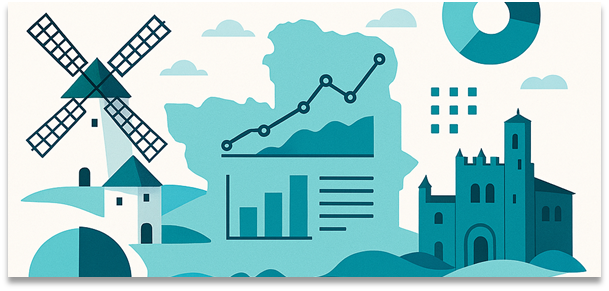
\includegraphics[width=0.8\textwidth,height=\textheight]{cover_ejemplo.png}

\bookmarksetup{startatroot}

\hypertarget{ciencia-y-tecnologuxeda}{%
\chapter{Ciencia y tecnología}\label{ciencia-y-tecnologuxeda}}

\hypertarget{estaduxedsticas-sobre-actividades-de-id}{%
\section{Estadísticas sobre actividades de
I+D}\label{estaduxedsticas-sobre-actividades-de-id}}

{\textbf{En 2023, CLM destinó un total de 332,8 millones de euros a
gastos en I+D interna}}\\
Esta cifra representa un 1,49\% del total nacional (22.379 millones de
euros).

\begin{table}[!h]
\centering
\caption{Gastos en I+D interna por sector en CLM (2023)}
\centering
\begin{tabular}[t]{lrr}
\toprule
\cellcolor[HTML]{FFF2CC}{Sector} & \cellcolor[HTML]{FFF2CC}{Gasto} & \cellcolor[HTML]{FFF2CC}{Porcentaje}\\
\midrule
\cellcolor{gray!10}{Adm. Públicas} & \cellcolor{gray!10}{51041} & \cellcolor{gray!10}{15.34}\\
Enseñanza Superior & 91150 & 27.39\\
\cellcolor{gray!10}{Empresas} & \cellcolor{gray!10}{190075} & \cellcolor{gray!10}{57.11}\\
IPSFL & 565 & 0.17\\
\cellcolor{gray!10}{Total} & \cellcolor{gray!10}{332831} & \cellcolor{gray!10}{100.00}\\
\bottomrule
\end{tabular}
\end{table}

\begin{tcolorbox}[enhanced jigsaw, leftrule=.75mm, breakable, toptitle=1mm, colframe=quarto-callout-note-color-frame, left=2mm, colback=white, bottomrule=.15mm, title=\textcolor{quarto-callout-note-color}{\faInfo}\hspace{0.5em}{El sector empresarial concentra el mayor esfuerzo en I+D en CLM.}, arc=.35mm, coltitle=black, colbacktitle=quarto-callout-note-color!10!white, toprule=.15mm, bottomtitle=1mm, opacityback=0, titlerule=0mm, rightrule=.15mm, opacitybacktitle=0.6]

Absorbe el 57,1\% del gasto, seguido por la enseñanza superior (27,4\%)
y las administraciones públicas (15,3\%).

\end{tcolorbox}

{\textbf{CLM presenta una mayor intensidad de innovación que la media
nacional en el conjunto de empresas (0.93 frente a 0.75)}}

Sin embargo, se sitúa por debajo en las empresas con gasto en innovación
(1.61 frente a 1.80) y en aquellas con actividades de I+D (1,90 frente a
2,75).

\begin{figure}

{\centering 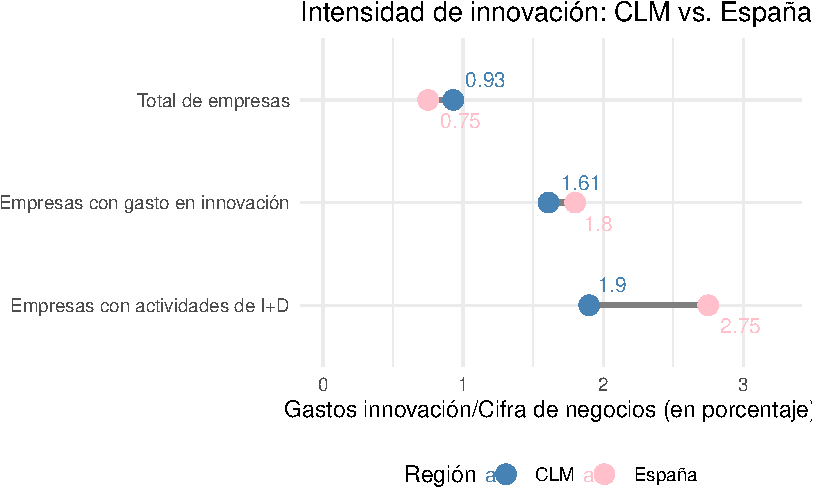
\includegraphics{clm01_ciencia_tecnologia_files/figure-pdf/lollipop-innovacion-1.pdf}

}

\caption{Intensidad de Innovación: España vs.~CLM. Fuente: INE (2022)}

\end{figure}

CLM presenta una mayor intensidad de innovación que la media nacional en
el conjunto de empresas (0.93 frente a 0.75). Sin embargo, se sitúa por
debajo en las empresas con gasto en innovación (1,61 frente a 1,80) y en
aquellas con actividades de I+D (1,90 frente a 2,75), lo que sugiere una
menor especialización en innovación avanzada.

\hypertarget{telecomunicaciones}{%
\section{Telecomunicaciones}\label{telecomunicaciones}}

\textbf{CLM avanza en digitalización con más de 98 líneas móviles por
cada 100 habitantes. Guadalajara y Toledo impulsan la conectividad en la
región con los mejores datos en banda ancha y telefonía fija. (a elegir
uno)}

\begin{tcolorbox}[enhanced jigsaw, leftrule=.75mm, breakable, toptitle=1mm, colframe=quarto-callout-note-color-frame, left=2mm, colback=white, bottomrule=.15mm, title=\textcolor{quarto-callout-note-color}{\faInfo}\hspace{0.5em}{CLM avanza en digitalización con más de 98 líneas móviles por cada 100
habitantes.}, arc=.35mm, coltitle=black, colbacktitle=quarto-callout-note-color!10!white, toprule=.15mm, bottomtitle=1mm, opacityback=0, titlerule=0mm, rightrule=.15mm, opacitybacktitle=0.6]

Guadalajara y Toledo impulsan la conectividad en la región con los
mejores datos en banda ancha y telefonía fija.

\end{tcolorbox}

\begin{figure}

{\centering 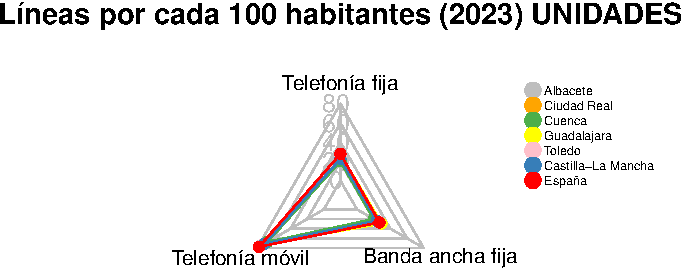
\includegraphics{clm01_ciencia_tecnologia_files/figure-pdf/teleco-clm-1.pdf}

}

\caption{Líneas telefónicas por cada 100 habitantes en CLM (2023)}

\end{figure}

\begin{itemize}
\item
  La televisión de pago en CLM alcanza 11,5 abonados/100 habitantes,
  ligeramente inferior a la que presenta España 14,3. La provincia con
  mayor penetración es Guadalajara (15,7), mientras que Albacete (8,1)
  presenta la menor proporción de abonados.
\item
  CLM cuenta con 3.983.928 accesos NGA instalados, siendo Toledo
  (1.288.366) la provincia con mayor número de accesos, mientras que
  Cuenca (434.912) presenta la menor cobertura. Comparando con España,
  CLM representa aproximadamente un 4,6\% del total nacional, indicando
  que, aunque la infraestructura es significativa, su peso relativo
  frente al conjunto del país es reducido.
\end{itemize}

\hypertarget{uso-de-las-tic-en-empresas}{%
\section{Uso de las TIC en empresas}\label{uso-de-las-tic-en-empresas}}

El 99,7\% de las empresas de CLM tienen ordenadores, pero solo el 49.6\%
del personal los usa con Internet

Solo el 55.8\,\% del personal utiliza ordenadores con fines
empresariales (frente al 68.4\,\% en España), y apenas el 49,6\% accede
a Internet con fines laborales (frente al 63,3\%).

\begin{tcolorbox}[enhanced jigsaw, leftrule=.75mm, breakable, toptitle=1mm, colframe=quarto-callout-note-color-frame, left=2mm, colback=white, bottomrule=.15mm, title=\textcolor{quarto-callout-note-color}{\faInfo}\hspace{0.5em}{Transformación digital y adopción tecnológica}, arc=.35mm, coltitle=black, colbacktitle=quarto-callout-note-color!10!white, toprule=.15mm, bottomtitle=1mm, opacityback=0, titlerule=0mm, rightrule=.15mm, opacitybacktitle=0.6]

La conexión a Internet alcanza a casi el 99\% de las empresas en CLM

\end{tcolorbox}

El 75,9\% de las empresas cuentan con sitio web, pero solo el 21,2\%
realizan analítica de datos internamente y apenas el 7,6\% emplean
inteligencia artificial, lo que evidencia una fuerte presencia digital
básica pero una baja adopción de tecnologías avanzadas.

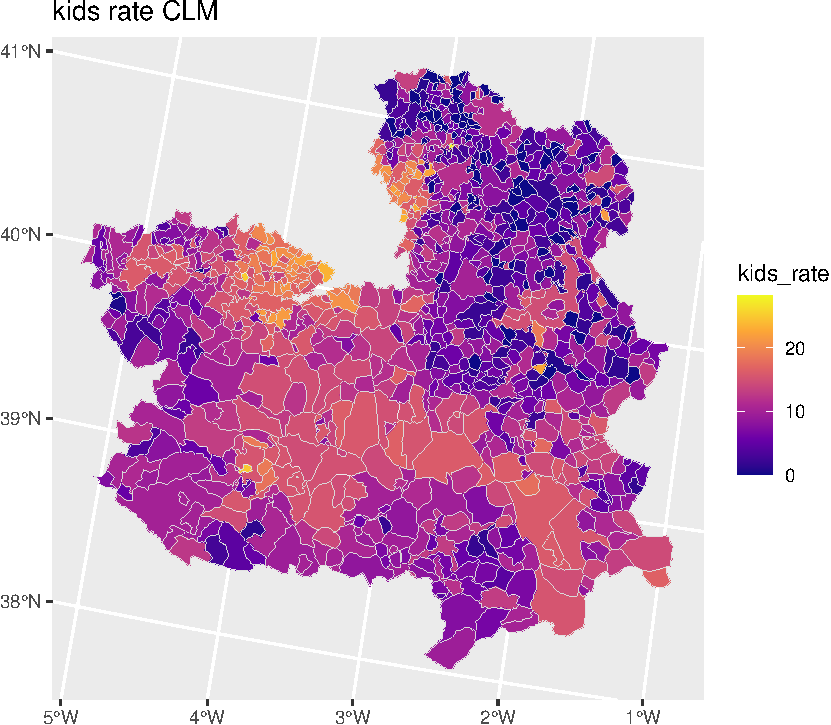
\includegraphics{clm01_ciencia_tecnologia_files/figure-pdf/unnamed-chunk-5-1.pdf}

\begin{tcolorbox}[enhanced jigsaw, leftrule=.75mm, breakable, toptitle=1mm, colframe=quarto-callout-note-color-frame, left=2mm, colback=white, bottomrule=.15mm, title=\textcolor{quarto-callout-note-color}{\faInfo}\hspace{0.5em}{Nota}, arc=.35mm, coltitle=black, colbacktitle=quarto-callout-note-color!10!white, toprule=.15mm, bottomtitle=1mm, opacityback=0, titlerule=0mm, rightrule=.15mm, opacitybacktitle=0.6]

\textbf{Unicamente el 5,95\% de los trabajadores teletrabaja de manera
regular.}

\end{tcolorbox}

\textbackslash begin\{table\}{[}!h{]} \centering
\textbackslash caption\{\label{tab:tabla-tic-especialistas}Indicadores
sobre especialistas en TIC en empresas (\%)\} \centering

\begin{table}
\caption{Indicadores sobre especialistas en TIC en empresas (\%)}\tabularnewline

\centering
\begin{tabular}[t]{lrr}
\toprule
\cellcolor[HTML]{FFF2CC}{Indicador} & \cellcolor[HTML]{FFF2CC}{CLM (\%)} & \cellcolor[HTML]{FFF2CC}{España (\%)}\\
\midrule
\cellcolor{gray!10}{Empresas que emplean especialistas en TIC*} & \cellcolor{gray!10}{8.48} & \cellcolor{gray!10}{15.67}\\
Empresas con mujeres especialistas TIC*** & 45.92 & 41.92\\
\cellcolor{gray!10}{Personal especialista TIC****} & \cellcolor{gray!10}{1.27} & \cellcolor{gray!10}{4.49}\\
\bottomrule
\end{tabular}
\end{table}

\textbackslash end\{table\}

\bookmarksetup{startatroot}

\hypertarget{comercio}{%
\chapter{Comercio}\label{comercio}}

\bookmarksetup{startatroot}

\hypertarget{cultura-y-ocio}{%
\chapter{Cultura y ocio}\label{cultura-y-ocio}}

\bookmarksetup{startatroot}

\hypertarget{demografuxeda}{%
\chapter{Demografía}\label{demografuxeda}}

\bookmarksetup{startatroot}

\hypertarget{deporte}{%
\chapter{Deporte}\label{deporte}}

\bookmarksetup{startatroot}

\hypertarget{economuxeda}{%
\chapter{Economía}\label{economuxeda}}

\bookmarksetup{startatroot}

\hypertarget{educaciuxf3n}{%
\chapter{Educación}\label{educaciuxf3n}}

\bookmarksetup{startatroot}

\hypertarget{empleo}{%
\chapter{Empleo}\label{empleo}}

\bookmarksetup{startatroot}

\hypertarget{energuxeda}{%
\chapter{Energía}\label{energuxeda}}

\bookmarksetup{startatroot}

\hypertarget{hacienda}{%
\chapter{Hacienda}\label{hacienda}}

\bookmarksetup{startatroot}

\hypertarget{industria}{%
\chapter{Industria}\label{industria}}

\bookmarksetup{startatroot}

\hypertarget{legislaciuxf3n-y-justicia}{%
\chapter{Legislación y justicia}\label{legislaciuxf3n-y-justicia}}

\bookmarksetup{startatroot}

\hypertarget{medio-ambiente}{%
\chapter{Medio ambiente}\label{medio-ambiente}}

\bookmarksetup{startatroot}

\hypertarget{medio-rural}{%
\chapter{Medio rural}\label{medio-rural}}

\bookmarksetup{startatroot}

\hypertarget{salud}{%
\chapter{Salud}\label{salud}}

\bookmarksetup{startatroot}

\hypertarget{sector-puxfablico}{%
\chapter{Sector público}\label{sector-puxfablico}}

\bookmarksetup{startatroot}

\hypertarget{seguridad}{%
\chapter{Seguridad}\label{seguridad}}

\bookmarksetup{startatroot}

\hypertarget{sociedad-y-bienestar}{%
\chapter{Sociedad y bienestar}\label{sociedad-y-bienestar}}

\bookmarksetup{startatroot}

\hypertarget{transporte}{%
\chapter{Transporte}\label{transporte}}

\bookmarksetup{startatroot}

\hypertarget{turismo}{%
\chapter{Turismo}\label{turismo}}

\bookmarksetup{startatroot}

\hypertarget{urbanismo-e-infraestructuras}{%
\chapter{Urbanismo e
infraestructuras}\label{urbanismo-e-infraestructuras}}

\bookmarksetup{startatroot}

\hypertarget{vivienda}{%
\chapter{Vivienda}\label{vivienda}}



\end{document}
